\documentclass[preprint,12pt]{elsarticle}

\usepackage{graphicx}
\usepackage{booktabs}
\usepackage{amsmath,amssymb}
\usepackage{hyperref}
\usepackage{multirow}
\usepackage{float}
\usepackage{tabularx}
\usepackage{makecell}

\journal{Applied Energy}

\newcolumntype{Y}{>{\centering\arraybackslash}X}
\begin{document}

\begin{frontmatter}

\title{Cost–Resilience Thresholds for Battery–Hydrogen Hybrid Microgrids in Islanded Power Systems: An 8760-h Real-Weather Philippines Study}

\author{Jaewon Lee}
\address{National Institute of Green Technology, Republic of Korea}

\begin{abstract}
This study examines when battery–hydrogen hybrid microgrids become economically defensible in islanded power systems under long-duration resilience requirements. Rather than performing endogenous capacity expansion, the paper adopts a fixed-capacity 8760-h operational screening framework that combines chronological real-weather dispatch with outage-focused resilience assessment for a representative off-grid Philippines archetype. Three portfolios are compared: battery-only, diesel-battery, and battery-hydrogen.

In the base case, diesel-battery is the least-cost option at 2.26 MUSD/yr (217.0 USD/MWh), but it serves only 64.3\% of critical load during modeled outages and survives only 3 h under the base outage setting. Battery-hydrogen raises annual cost to 6.35 MUSD/yr (610.5 USD/MWh), but maintains full critical-load service for 48-h outages while eliminating diesel-related CO2 emissions. Battery-only also maintains full critical-load service during outages under the present fixed-capacity setting, but incurs annual unmet load and the highest total system cost.

A structured threshold screening across delivered diesel cost, outage duration, hydrogen CAPEX, and carbon price shows that hydrogen is not a universally least-cost solution. Its value emerges when long outage duration, costly diesel logistics, carbon exposure, and lower hydrogen capital cost jointly shift the cost–resilience frontier. The contribution of the paper is therefore not to claim a globally optimal island design, but to identify the conditions under which hydrogen should be screened as a resilience-oriented long-duration resource in islanded microgrids.
\end{abstract}

\begin{keyword}
Islanded microgrid \sep Hydrogen storage \sep Resilience \sep Outage analysis \sep Long-duration storage \sep Techno-economic analysis \sep Critical load
\end{keyword}

\end{frontmatter}

\section{Introduction}
Remote islanded power systems face a fundamental trade-off between cost minimization and resilience under fuel logistics risk, renewable intermittency, and prolonged outages. While diesel-battery systems often remain cost-competitive, battery-hydrogen systems may become justified when long-duration resilience needs intensify. This study aims to identify the threshold conditions under which hydrogen coupling becomes economically defensible in islanded microgrids.
Existing studies on islanded microgrids have extensively examined photovoltaic-battery coordination, diesel displacement, and off-grid electrification in the Philippines and other remote settings, while a growing body of work has also explored hydrogen as a long-duration storage option in remote systems \cite{ocon_bertheau_2019_philippines_diesel_pvbatt,pascasio_2021_philippines_pv_wind,castro_2022_634_islands_hres,castro_2023_busuanga_resilience,castro_2024_208_islands_transition,salac_2024_philippines_offgrid_review,alzahrani_2022_hydrogen_microgrid_review,van_2023_hydrogen_microgrid_review,tatti_2024_hydrogen_offgrid_case}. More broadly, remote and islanded microgrid studies have highlighted the importance of logistics constraints, weather variability, and context-specific resilience requirements in isolated systems \cite{hirsch_2018_microgrids_review,akinyele_2018_remote_microgrid_challenges}. Recent hydrogen-microgrid research has also moved beyond generic integration concepts toward coordinated operation and extreme-event resilience \cite{huang_2023_economic_resilient_h2_microgrid,shahbazbegian_2023_resilience_p2h,sharifpour_2023_hydrogen_extreme_events,qi_2025_h2_battery_dispatch}. However, much of the literature remains limited in one of three ways. First, many studies evaluate hydrogen using stylized or annual-average conditions without preserving chronological hourly operating feasibility. Second, resilience is often treated qualitatively or through simplified reliability proxies without explicitly simulating outage survival under constrained local resources. Third, the economic value of hydrogen is frequently discussed in general terms, rather than expressed as a threshold condition jointly governed by diesel logistics cost, outage severity, carbon valuation, and hydrogen capital cost.

These limitations are particularly important in remote island systems. In such contexts, system design is shaped not only by average energy cost, but also by prolonged outages, fuel delivery uncertainty, weak operational flexibility, and critical-load survival requirements. As a result, hydrogen should not be assessed solely as an energy carrier or decarbonization option; it should also be evaluated as a resilience resource whose value may emerge only beyond specific operating thresholds.

This paper addresses a narrower but practically important question than full capacity expansion: under fixed candidate portfolio capacities and real-weather hourly operation, when does hydrogen materially shift the cost–resilience frontier of an islanded microgrid relative to diesel-based flexibility? To answer this, the study makes three contributions. First, it develops an 8760-h chronological operational framework for comparing battery-only, diesel-battery, and battery-hydrogen portfolios under common weather and demand assumptions. Second, it integrates outage-focused post-processing to quantify resilience using critical-load-served ratio, expected energy not served, and survivable outage duration. Third, it identifies the threshold conditions under which battery-hydrogen becomes economically defensible relative to diesel-battery as delivered diesel cost, outage severity, carbon price, and hydrogen CAPEX vary. The contribution is therefore an operational threshold screening framework for islanded systems, rather than an endogenous expansion-planning model or a feeder-specific utility planning study.
\section{Methodology}

This study evaluates whether hydrogen coupling changes the cost--resilience frontier of an islanded microgrid under realistic operating conditions. The analytical workflow consists of three sequential layers: (i) fixed-capacity hourly dispatch optimization over 8760 h, (ii) outage-focused resilience post-processing, and (iii) structured threshold sensitivity analysis \cite{qi_2025_h2_battery_dispatch,gao_2016_critical_load_restoration,raoufi_2020_power_resilience_metrics,amiri_2024_resilience_framework}. The framework is designed as an operational threshold study rather than a full capacity expansion model.

\subsection{System configuration and candidate portfolios}

Three candidate portfolios are considered: battery-only, diesel-battery, and battery-hydrogen. Across portfolios, photovoltaic generation is treated as the primary renewable source, while flexibility is provided by battery storage, diesel generation, and, where applicable, a hydrogen subsystem consisting of an electrolyzer, hydrogen storage tank, and fuel cell. Technology capacities are fixed ex ante for each candidate portfolio so that the analysis can isolate differences in hourly operational feasibility and resilience behavior under common case assumptions. The fixed portfolio definitions are summarized in Supplementary Table~S1.

\subsection{Hourly dispatch optimization}

For each portfolio, hourly dispatch is formulated as a linear cost-minimization problem over $t \in \{1,\dots,8760\}$:
\begin{equation}
\min \; C^{\mathrm{ann}}
=
C^{\mathrm{cap,ann}} + C^{\mathrm{fix}} + C^{\mathrm{var}} + C^{\mathrm{diesel}} + C^{\mathrm{carbon}} + C^{\mathrm{unserved}},
\end{equation}
where $C^{\mathrm{cap,ann}}$ is annualized capital cost, $C^{\mathrm{fix}}$ is fixed operation and maintenance cost, $C^{\mathrm{var}}$ is variable operating cost, $C^{\mathrm{diesel}}$ is delivered diesel fuel cost, $C^{\mathrm{carbon}}$ is the carbon price applied to diesel-related emissions, and $C^{\mathrm{unserved}}$ is the unmet-load penalty.

Hourly power balance is enforced as
\begin{equation}
P^{\mathrm{PV}}_t + P^{\mathrm{diesel}}_t + P^{\mathrm{bat,dis}}_t + P^{\mathrm{fc}}_t + P^{\mathrm{unserved}}_t
=
L_t + P^{\mathrm{bat,ch}}_t + P^{\mathrm{ely}}_t,
\end{equation}
where $P^{\mathrm{PV}}_t$ is photovoltaic generation, $P^{\mathrm{diesel}}_t$ is diesel generation, $P^{\mathrm{bat,dis}}_t$ and $P^{\mathrm{bat,ch}}_t$ are battery discharge and charge, $P^{\mathrm{fc}}_t$ is fuel-cell output, $P^{\mathrm{ely}}_t$ is electrolyzer electricity consumption, $L_t$ is hourly load, and $P^{\mathrm{unserved}}_t$ is unmet load.

\subsection{Battery and hydrogen state equations}

Battery state of charge evolves according to
\begin{equation}
E^{\mathrm{bat}}_t
=
E^{\mathrm{bat}}_{t-1}
+ \eta^{\mathrm{ch}}_{\mathrm{bat}} P^{\mathrm{bat,ch}}_t \Delta t
-
\frac{P^{\mathrm{bat,dis}}_t \Delta t}{\eta^{\mathrm{dis}}_{\mathrm{bat}}},
\end{equation}
subject to
\begin{equation}
E^{\mathrm{bat,min}} \le E^{\mathrm{bat}}_t \le E^{\mathrm{bat,max}}.
\end{equation}

Hydrogen inventory evolves according to
\begin{equation}
H_t
=
H_{t-1}
+ \eta_{\mathrm{ely}} P^{\mathrm{ely}}_t \Delta t
-
\frac{P^{\mathrm{fc}}_t \Delta t}{\eta_{\mathrm{fc}}},
\end{equation}
subject to
\begin{equation}
H^{\min} \le H_t \le H^{\max}.
\end{equation}

A cyclic annual boundary condition is imposed on both storage states so that the final-hour storage level equals the initial storage level.

\subsection{Outage-focused resilience assessment}

Resilience is assessed in a post-dispatch outage simulation rather than embedded directly in the annual dispatch objective. A set of outage events is generated according to the configured outage frequency, outage duration, and random seed. During outage events, diesel generation is disabled in the base resilience setting, and the system must serve the critical-load profile
\begin{equation}
L^{\mathrm{crit}}_t = \alpha L_t,
\end{equation}
where $\alpha$ denotes the critical-load fraction.

The critical-load-served ratio (CLSR) is defined as
\begin{equation}
\mathrm{CLSR}
=
\frac{\sum_{e}\sum_{t \in e} \left(L^{\mathrm{crit}}_t - P^{\mathrm{crit,unserved}}_t\right)}
{\sum_{e}\sum_{t \in e} L^{\mathrm{crit}}_t }.
\end{equation}

Expected energy not served during outages is defined as
\begin{equation}
\mathrm{EENS}
=
\sum_{e}\sum_{t \in e} P^{\mathrm{crit,unserved}}_t \Delta t.
\end{equation}

Survivable outage duration is defined as the maximum contiguous outage duration for which the portfolio maintains full critical-load service under the stated outage simulation setting.

\subsection{Threshold sensitivity design}

Threshold behavior is explored by varying four exogenous dimensions: delivered diesel cost, outage duration, hydrogen CAPEX multiplier, and carbon price. Each sensitivity case is solved independently under the same model structure. The purpose of the sensitivity analysis is not to identify a globally optimal design, but to determine the parameter regions in which battery-hydrogen becomes economically defensible relative to diesel-battery on the cost--resilience frontier. The rationale for the screened parameter ranges is summarized in Supplementary Table~S4.

The use of fixed candidate capacities is a deliberate design choice intended to isolate operational and resilience threshold behavior across comparable portfolios under common assumptions, rather than to claim globally optimal technology sizing.

\subsection{Implementation and reproducibility}

The optimization model was implemented in Python and solved as a linear program at hourly resolution over 8760 time steps for each candidate portfolio and sensitivity case. All scenarios were evaluated using a consistent input structure, common time resolution, cyclic storage boundary conditions, and fixed random seeds for outage sampling. The input assumptions, scenario definitions, and output tables used to generate the reported results are documented in the Supplementary Material. A repository-ready file structure and README are also prepared for public release as referenced in the Data Availability Statement.

\section{Case study and assumptions}
\begin{table}[H]
\centering
\caption{Case study assumptions for the representative Philippines off-grid island system.}
\label{tab:assumptions}
\begin{tabular}{p{5.2cm} p{8.8cm}}
\toprule
Item & Value / description \\
\midrule
Country / context & Philippines; representative off-grid island or remote distribution area \\
Weather source & NASA POWER hourly data (2025), point-based real-weather input \\
Analysis year & 2025 \\
Time resolution & 1 hour (8760 hours) \\
Load representation & Calibrated synthetic island load archetype \\
Peak demand & 1.65 MW \\
Load factor & 0.72 \\
Evening peak strength & 0.30 \\
Morning peak strength & 0.10 \\
Commercial load fraction & 0.14 \\
Seasonal multiplier & Monthly profile specified in the scenario configuration \\
Tourism load effect & Peak months: March, April, December; multiplier 1.08 \\
Critical load fraction & 0.55 \\
Outage frequency & 4 events/year \\
Outage duration & 48 h in the base resilience setting; varied in sensitivity analysis \\
Diesel availability during outage & Not available during modeled outage events \\
Carbon price (base) & 0 USD/tCO$_2$ \\
Carbon price range & 0, 150, 300 USD/tCO$_2$ \\
Delivered diesel cost range & 180, 380, 700 USD/MWh \\
Hydrogen CAPEX multiplier range & 0.45, 0.70, 1.00 \\
Compared portfolios & Battery-only, diesel-battery, battery-hydrogen \\
Optimization scope & Fixed-capacity hourly dispatch optimization with resilience post-processing \\
\bottomrule
\end{tabular}
\end{table}

The case is intended as a representative off-grid island archetype rather than a site-specific utility planning model. The objective is to test operational threshold behavior under realistic weather and island-like demand characteristics, not to reproduce the exact dispatch history of a licensed feeder. The synthetic load profile is therefore used as a transparent and calibrated demand representation defined by peak demand, load factor, diurnal structure, commercial share, and seasonal modifiers, allowing the threshold behavior of alternative flexibility portfolios to be examined without implying feeder-specific universality.

The calibrated synthetic load archetype is used to preserve transparency and portability of the threshold analysis. The purpose is not to replicate a specific feeder’s dispatch history, but to test whether the threshold logic persists under island-like demand characteristics defined by peak demand, load factor, diurnal structure, commercial share, and seasonal modifiers. The load-construction rules and representative monthly and daily characteristics are documented in Supplementary Section~S2.

\section{Results}

\begin{table}[H]
\centering
\footnotesize
\setlength{\tabcolsep}{4pt}
\caption{Comparison of the three candidate portfolios in the real-weather Philippines case study.}
\label{tab:mainresults}
\begin{tabularx}{\textwidth}{p{2.6cm}YYYYYYY}
\toprule
\makecell[c]{Scenario} &
\makecell[c]{Annual cost\\(MUSD/yr)} &
\makecell[c]{LCOE\\(USD/MWh)} &
\makecell[c]{Diesel CO$_2$\\(t/yr)} &
\makecell[c]{Unmet load\\(MWh/yr)} &
\makecell[c]{Critical load\\served ratio (-)} &
\makecell[c]{EENS\\(MWh)} &
\makecell[c]{Survivable outage\\duration (h)} \\
\midrule
Battery-only     & 21.25 & 2511.4 & 0.0    & 44.5 & 1.000 & 0.0  & 48 \\
Diesel-battery   & 2.26  & 217.0  & 4564.0 & 0.0  & 0.643 & 45.7 & 3  \\
Battery-hydrogen & 6.35  & 610.5  & 0.0    & 0.0  & 1.000 & 0.0  & 48 \\
\bottomrule
\end{tabularx}
\end{table}

Note: Annual unmet load is evaluated against full-load service over all operating hours, whereas CLSR, EENS, and survivable outage duration are evaluated only during modeled outage windows and only for the critical-load fraction. Accordingly, a portfolio may maintain full critical-load service during outages while still incurring annual unmet load under full-demand operation.


Table~\ref{tab:mainresults} reveals three distinct portfolio roles. The diesel-battery configuration is the least-cost option in the base case, with an annual cost of 2.26 MUSD/yr and an LCOE of 217.0 USD/MWh, but it shows substantially weaker outage resilience, serving only 64.3\% of critical load during modeled outage events, with 45.7 MWh of EENS and a survivable outage duration of only 3 h. By contrast, the battery-hydrogen configuration increases annual cost to 6.35 MUSD/yr, but eliminates diesel-related CO$_2$ emissions, removes annual unmet load, and maintains full critical-load service for 48 h outages. The battery-only configuration also maintains full critical-load service during the modeled outage events, but it exhibits 44.5 MWh of annual unmet load and the highest system cost, indicating that under the present sizing assumptions it is not an economically credible full-load benchmark. These results suggest that hydrogen should not be interpreted as a universally least-cost option, but rather as a resilience-oriented alternative to diesel-based flexibility in high-risk island operating conditions.

It is important to distinguish the annual service metric from the outage-specific resilience metrics. Annual unmet load is evaluated with respect to full-load service across all operating hours, whereas critical-load-served ratio, EENS, and survivable outage duration are evaluated only during modeled outage windows and only for the critical-load fraction. Accordingly, the battery-only case can maintain full critical-load service during outage events while still failing to serve full annual demand under the present fixed-capacity assumptions.

\subsection{Cost--resilience trade-off}
Fig.~\ref{fig:tradeoff} shows the cost--resilience trade-off between diesel-battery and battery-hydrogen portfolios. Battery-hydrogen maintains full critical-load service across sensitivity cases, while diesel-battery remains cost-competitive but systematically below full outage resilience.

\begin{figure}[H]
    \centering
    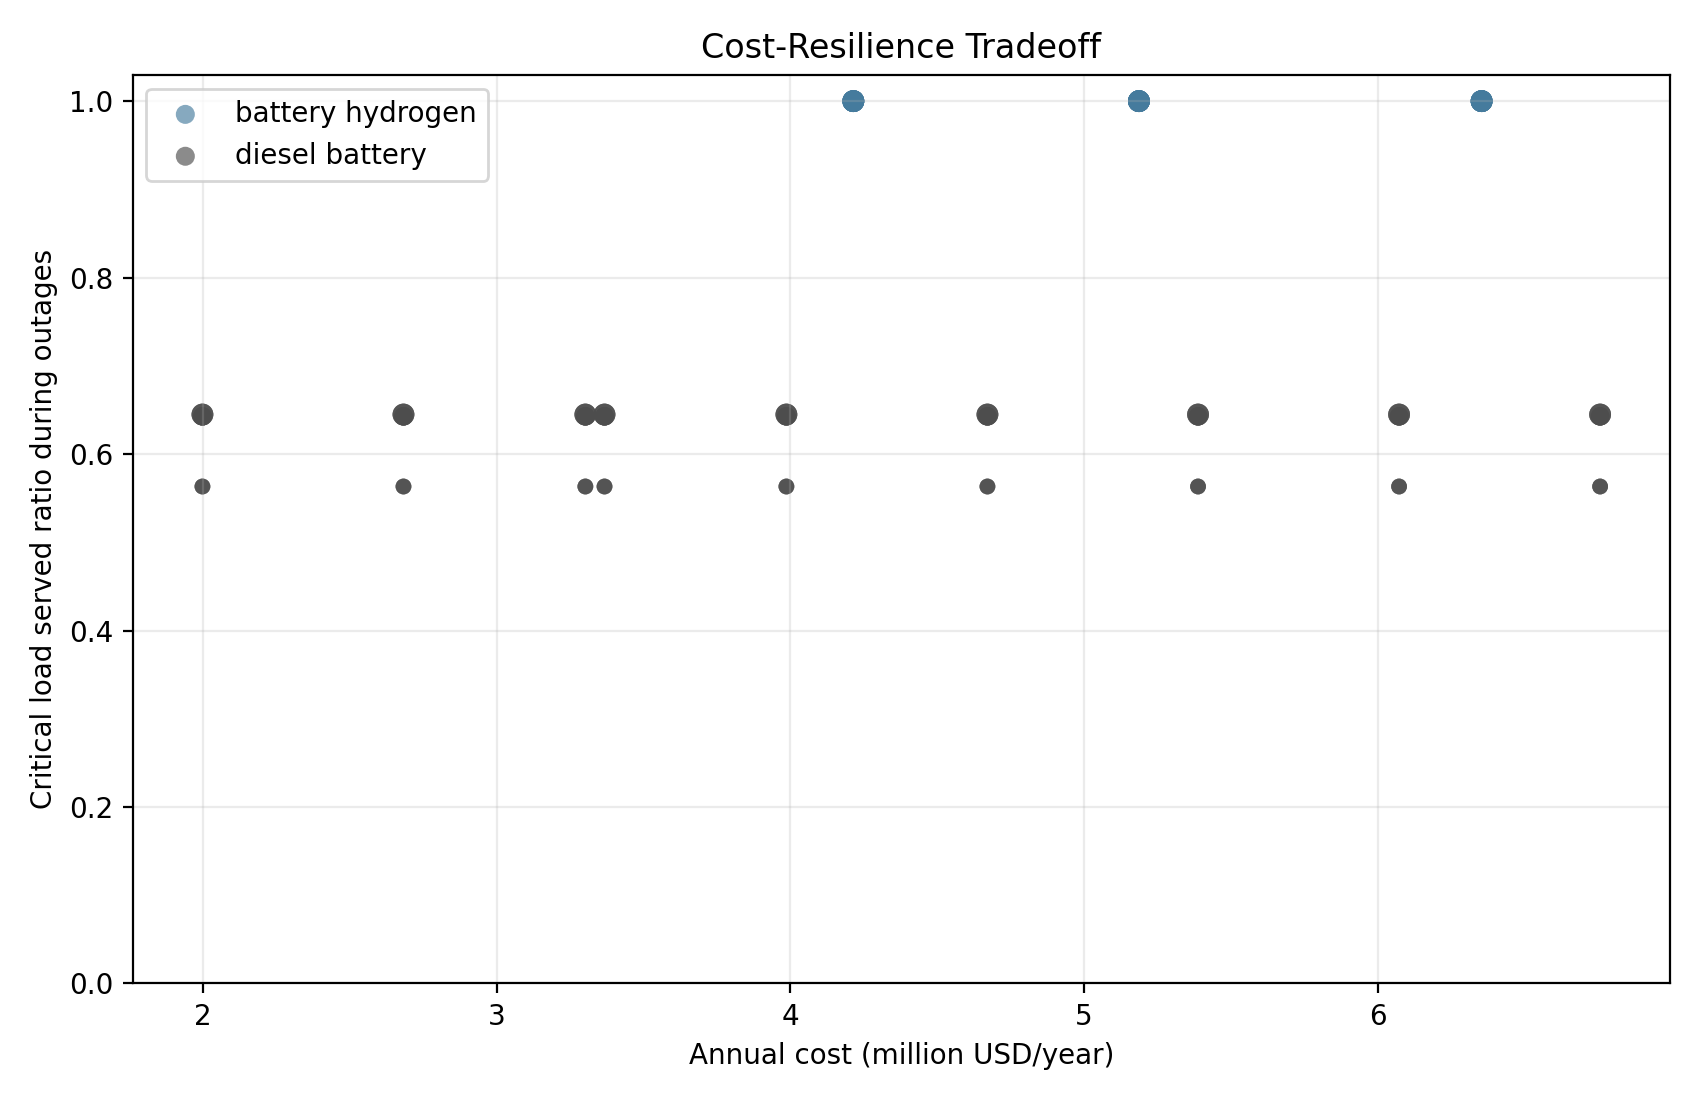
\includegraphics[width=0.78\textwidth]{figures/cost_resilience_tradeoff.png}
\caption{Cost--resilience trade-off between diesel-battery and battery-hydrogen portfolios across sensitivity cases. Battery-hydrogen maintains full critical-load service during modeled outages, whereas diesel-battery remains cost-competitive but systematically below full outage resilience.}    \label{fig:tradeoff}
\end{figure}

\subsection{Hydrogen threshold conditions}
Fig.~\ref{fig:threshold} presents the annual cost difference of battery-hydrogen relative to diesel-battery under the 48-h outage screening condition and a carbon price of 150 USD/tCO$_2$. Negative values indicate cases in which battery-hydrogen achieves lower annual cost than diesel-battery under the specified screening setting.

\begin{figure}[H]
    \centering
    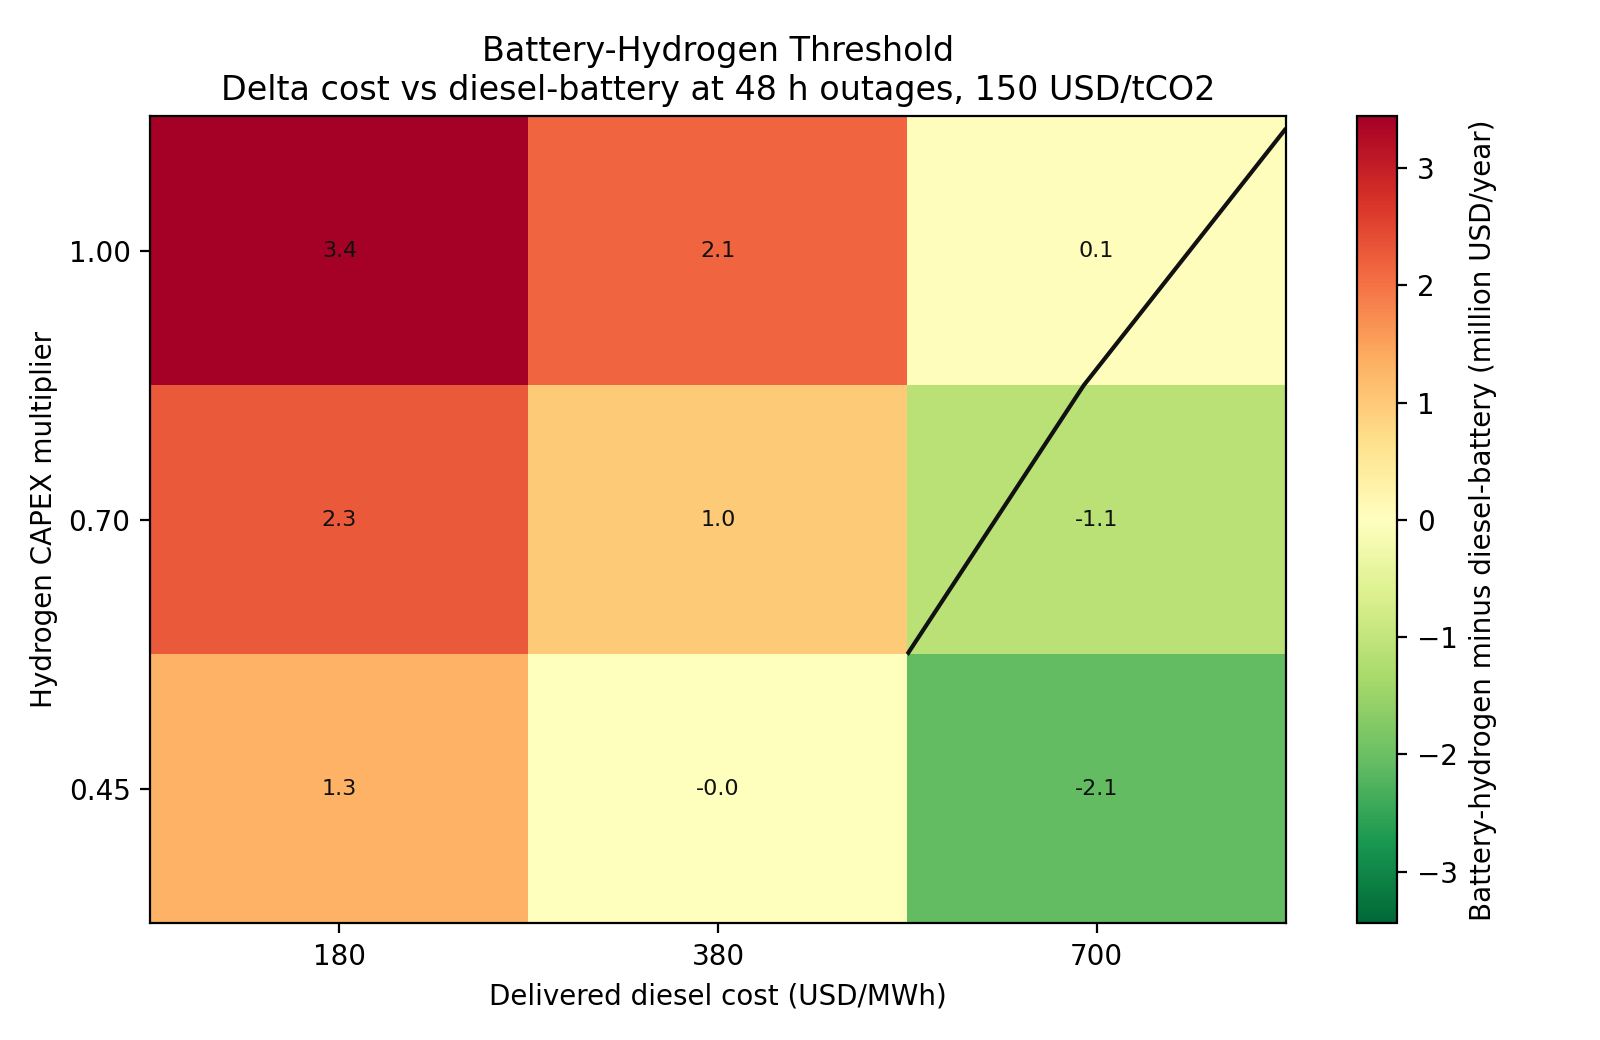
\includegraphics[width=0.78\textwidth]{figures/threshold_heatmap.png}
    \caption{Threshold conditions under which battery-hydrogen becomes economically preferable to diesel-battery under the 48-h outage screening condition and a carbon price of 150 USD/tCO$_2$. Negative values indicate cases in which battery-hydrogen yields lower annual cost than diesel-battery.}
    \label{fig:threshold}
\end{figure}

The results indicate that battery-hydrogen is not universally optimal, but becomes economically defensible as delivered diesel cost rises and hydrogen CAPEX declines. This confirms that hydrogen viability in islanded systems is governed by identifiable threshold conditions rather than average-cost logic alone.

\section{Discussion}

\subsection{Implications for islanded system planning}

The results suggest that hydrogen should not be evaluated in islanded systems primarily through average-cost superiority. In the present case, diesel-battery remains the least-cost benchmark in the base case, whereas battery-hydrogen changes the resilience envelope by maintaining full critical-load service during severe modeled outages. The planning implication is therefore not that hydrogen replaces diesel in all island contexts, but that hydrogen becomes defensible when the operational environment is shaped by long outage duration, costly fuel delivery, or stronger carbon constraints \cite{tatti_2024_hydrogen_offgrid_case,huang_2023_economic_resilient_h2_microgrid,shahbazbegian_2023_resilience_p2h,staadecker_2024_ldes_value}. In this sense, hydrogen acts as a contingency-oriented long-duration flexibility option rather than a universal least-cost resource.

This threshold-based interpretation is particularly relevant for remote island systems in which resilience failures create disproportionate social and economic consequences. For such systems, planning decisions based only on average annual cost can understate the value of long-duration resources that are rarely used in normal operation but become decisive during high-impact contingency periods.

From a planning perspective, the relevant question is not whether hydrogen outperforms diesel on average annual cost alone, but whether the operating environment is severe enough that resilience value justifies a higher-cost portfolio. The results suggest a practical screening logic for islanded systems. Where delivered diesel cost is moderate, outage duration is limited, and diesel backup remains dependable, diesel-battery is likely to remain the pragmatic benchmark. However, where prolonged outages, costly fuel logistics, carbon exposure, and declining hydrogen capital cost interact, average-cost rankings can understate the value of long-duration resilience. In such settings, hydrogen should be screened not as a universal diesel substitute, but as a threshold-dependent resilience resource.

\subsection{Study scope and limitations}

This paper is designed as an operational threshold study rather than a full capacity expansion study. Technology capacities are fixed ex ante so that the analysis can isolate how alternative portfolios behave under common weather, demand, and outage settings. Accordingly, the contribution is narrower than that of an endogenous sizing model: it does not claim a globally optimal island design, but instead identifies the boundary conditions under which hydrogen shifts the cost--resilience frontier relative to diesel-battery.

Diesel unavailability in the base outage setting is intended to represent severe fuel-logistics disruption during island contingency events rather than a universal operating condition. The assumption is therefore interpreted as a resilience stress case for threshold screening, not as a claim about all island outages. Supplementary Section~S3 provides the outage-setting rationale and a reviewer-facing robustness note.

The study is also based on a single representative Philippines case and a calibrated synthetic load archetype rather than measured feeder demand. These choices limit direct feeder-level generalization, but they do not invalidate the threshold logic of the analysis. The purpose is not to infer universal island-wide cost rankings from one site, but to show that hydrogen value is conditional and emerges beyond identifiable combinations of outage severity, diesel logistics cost, carbon price, and hydrogen capital cost. These limitations narrow the scope of generalization, but they do not alter the central contribution of the paper: identifying threshold-dependent resilience value under a transparent operational screening framework. Future work should extend the framework through multi-year weather testing, load-side robustness checks, endogenous sizing, and additional island cases.

\section{Conclusion}

This study assessed three fixed-capacity microgrid portfolios---battery-only, diesel-battery, and battery-hydrogen---for a representative off-grid Philippines case under real-weather hourly operation and outage-focused resilience assessment. The results show that battery-hydrogen is not the least-cost option in the base case, but becomes economically defensible when diesel cost, outage severity, carbon price, and hydrogen CAPEX jointly cross identifiable threshold conditions. The practical implication is that hydrogen should not be judged in islanded microgrids by average-cost comparison alone. Instead, it should be evaluated as a threshold-dependent long-duration resilience resource whose value emerges when outage risk, diesel logistics cost, carbon exposure, and hydrogen cost conditions jointly become severe enough to justify paying for resilience.

\section*{Data availability}

The code, scenario definitions, processed output tables, and supplementary materials required to reproduce the reported findings are publicly archived at https://doi.org/10.5281/zenodo.19658748, with version-controlled source files maintained at https://github.com/exoprime-sketch/microgrid-h2-paper.

\section*{Declaration of competing interest}

The author declares that he has no known competing financial interests or personal relationships that could have appeared to influence the work reported in this paper.

\section*{Funding}

This research did not receive any specific grant from funding agencies in the public, commercial, or not-for-profit sectors.

\section*{Declaration of generative AI and AI-assisted technologies in the manuscript preparation process}

During the preparation of this work, the author used generative AI tools to improve language clarity and manuscript organization. After using these tools, the author reviewed and edited the content as needed and takes full responsibility for the content of the published article.

\bibliographystyle{elsarticle-num}
\bibliography{refs}

\end{document}